\documentclass[conference]{IEEEtran}
\IEEEoverridecommandlockouts

\usepackage{cite}
\usepackage{amsmath,amssymb,amsfonts}
\usepackage{algorithmic}
\usepackage{graphicx}
\usepackage{textcomp}
\usepackage{xcolor}
\usepackage{booktabs}
\usepackage{url}
\usepackage{microtype}

\begin{document}

\title{Adaptive Client Selection for Concept Drift in Federated Learning}

\author{
\IEEEauthorblockN{Anonymous Authors}
\IEEEauthorblockA{Paper Under Double-Blind Review for ICACS}
}

\maketitle

\begin{abstract}
Edge devices in federated learning don't keep stationary data distributions over long deployment horizons. They face sudden concept shifts, sensor degradation, and seasonal label variations. Under standard bandwidth limits, a central server only talks to a small fraction of clients in each round. Unselected clients can't report their state, so the server doesn't observe them. Common greedy selection schemes pick the same top clients repeatedly. That causes severe client starvation, leaving most edge clients unselected. Stagnant clients don't get checked, so the system won't catch recovery when conditions change. This paper studies FedQual-CPX, an adaptive client selection framework for non-stationary federated networks. The system tracks local loss improvements, scales them with causal median absolute deviation normalization, and spots shifts using two-sided cumulative sum detectors. An adaptive exploration controller raises sampling rates when drift happens, while staleness scoring pulls forgotten clients back into training. Across experiments on CIFAR-10, FEMNIST, and Shakespeare with five random seeds, the proposed policy maintains full client participation. It cuts participation inequality by up to fifty-four percent compared to greedy selection and preserves post-drift recovery.
\end{abstract}

\begin{IEEEkeywords}
Federated learning, concept drift, client selection, change point detection, participation fairness.
\end{IEEEkeywords}

\section{Introduction}
Federated learning lets edge devices train a shared model without sending raw records to a central facility [1]. Smartphones, medical scanners, and connected vehicles compute updates locally and send parameter differences back to a coordination server [2]. But real edge deployments don't stay steady over time. Client data distributions drift because user habits change, lighting shifts, and physical sensors slowly degrade.

Partial observability makes client selection difficult under concept drift. The server doesn't see every client in every communication round. Bandwidth constraints force the server to pick only ten out of a hundred clients per round. When a client isn't picked, its current data distribution and loss gain stay completely hidden. A missing observation isn't a zero. It is simply unknown.

Prior selection methods struggle with this partial observability. Lai et al. [2] show that greedy utility sampling speeds up model training in static settings. Yet under concept drift, greedy selection traps the server in a narrow clique of previously strong devices. Stale clients don't get revisited, and newly improved clients can't show their worth. Li et al. [3] study optimization under device heterogeneity, but their setup doesn't handle temporal distribution shifts. Standard random selection explores every client evenly, but it doesn't exploit high-performing devices effectively.

Moving average filters and windowed methods also fall short. They smooth out utility fluctuations over fixed time frames, so they can't catch sudden drops quickly. By the time a moving window notices that a client drifted, the server has already integrated dozens of damaged updates. Heuristic restart rules like those in FLEX [5] try to clear outdated memory, but resetting the model throws away hard-won convergence progress. What edge networks need is an online selection rule that tracks client quality shifts directly.

This paper presents FedQual-CPX, an adaptive selection framework that explicitly handles partial observability under concept drift. Instead of relying on static rules, the server tracks loss improvements, flags distribution shifts with sequential cumulative sum tests, and adapts exploration rates dynamically. Neglected clients aren't abandoned. They get pulled back into training before selection biases harden.

The main findings of this work show three clear patterns:
\begin{enumerate}
    \item Greedy client selection collapses in non-stationary networks. It starves eighty to ninety percent of available devices and locks into high participation inequality.
    \item Sequential change detection paired with dynamic exploration restores full client coverage across all tested benchmarks without hurting global accuracy.
    \item Causal median absolute deviation scaling stabilizes utility tracking across diverse network architectures without leaking future observations.
\end{enumerate}

\section{Related Work}
Client selection has received wide attention in distributed machine learning. McMahan et al. [1] introduce federated averaging using uniform random participant sampling. Random sampling gives every device an equal selection chance, but it doesn't prioritize informative updates. Nishio and Yonetani [4] incorporate client compute and communication capabilities to prune stragglers. Lai et al. [2] formulate the Oort framework, selecting clients based on statistical utility and training speed. While Oort speeds up convergence under stationary data, it doesn't account for temporal shifts. It locks onto early high-utility devices and starves the remaining network.

Concept drift in edge networks poses distinct challenges. Lu et al. [5] and Gama et al. [6] categorize drift into abrupt, gradual, and incremental types. In centralized data streaming, drift detectors monitor loss streams directly. In federated networks, central servers can't inspect client data streams due to privacy rules and partial sampling. Recent efforts attempt to manage drift by clustering clients or restarting models. Model restarts disrupt ongoing optimization, and client clustering doesn't scale when individual device behaviors drift independently.

Sequential change-point analysis traces back to continuous inspection schemes. Page [7] introduces the cumulative sum (CUSUM) test to detect mean shifts in sequential observations. Basseville and Nikiforov [8] formalize two-sided detection for bounded false-alarm rates. While sequential detectors are common in industrial signal monitoring, their application to federated client selection remains rare. Existing federated drift handlers either use fixed exploration rates or rely on uncalibrated loss differences. FedQual-CPX bridges this gap by coupling sequential cumulative sum tracking with dynamic epistemic exploration.

\section{Problem Formulation}
A federated system trains over $N$ edge devices indexed by $i \in \{1, \dots, N\}$. Each device holds a local dataset $\mathcal{D}_{i,t}$ that may change across communication rounds $t \in \{1, \dots, T\}$. In round $t$, the server selects a cohort $S_t \subset \{1, \dots, N\}$ containing $|S_t| = K \ll N$ clients.

Clients in $S_t$ download global parameters $\mathbf{w}_t$, run local stochastic gradient descent for $E$ epochs, and upload local parameters $\mathbf{w}_{i,t}$. Following the formulation in McMahan et al. [1], the server aggregates parameter updates through sample-weighted averaging:
\begin{equation}
\mathbf{w}_{t+1} = \sum_{i \in S_t} \frac{n_i}{\sum_{j \in S_t} n_j} \mathbf{w}_{i,t}
\end{equation}

Raw gradient norms don't tell whether local training actually helped the global objective. This paper defines client utility as the empirical loss gain achieved locally:
\begin{equation}
u_{i,t} = \mathcal{L}_i(\mathbf{w}_t; \mathcal{D}_{i,t}) - \mathcal{L}_i(\mathbf{w}_{i,t}; \mathcal{D}_{i,t})
\end{equation}
A positive value $u_{i,t} > 0$ marks constructive progress. A negative value indicates harmful updates, such as corrupted labels or noise.

When client $i \notin S_t$, its utility isn't observed. The server doesn't set missing values to zero because doing so would mimic severe model degradation. Instead, the server maintains an explicit observation mask and tracks staleness counters. A missing observation simply means information is absent until that client is selected again.

\begin{figure}[t]
\centering
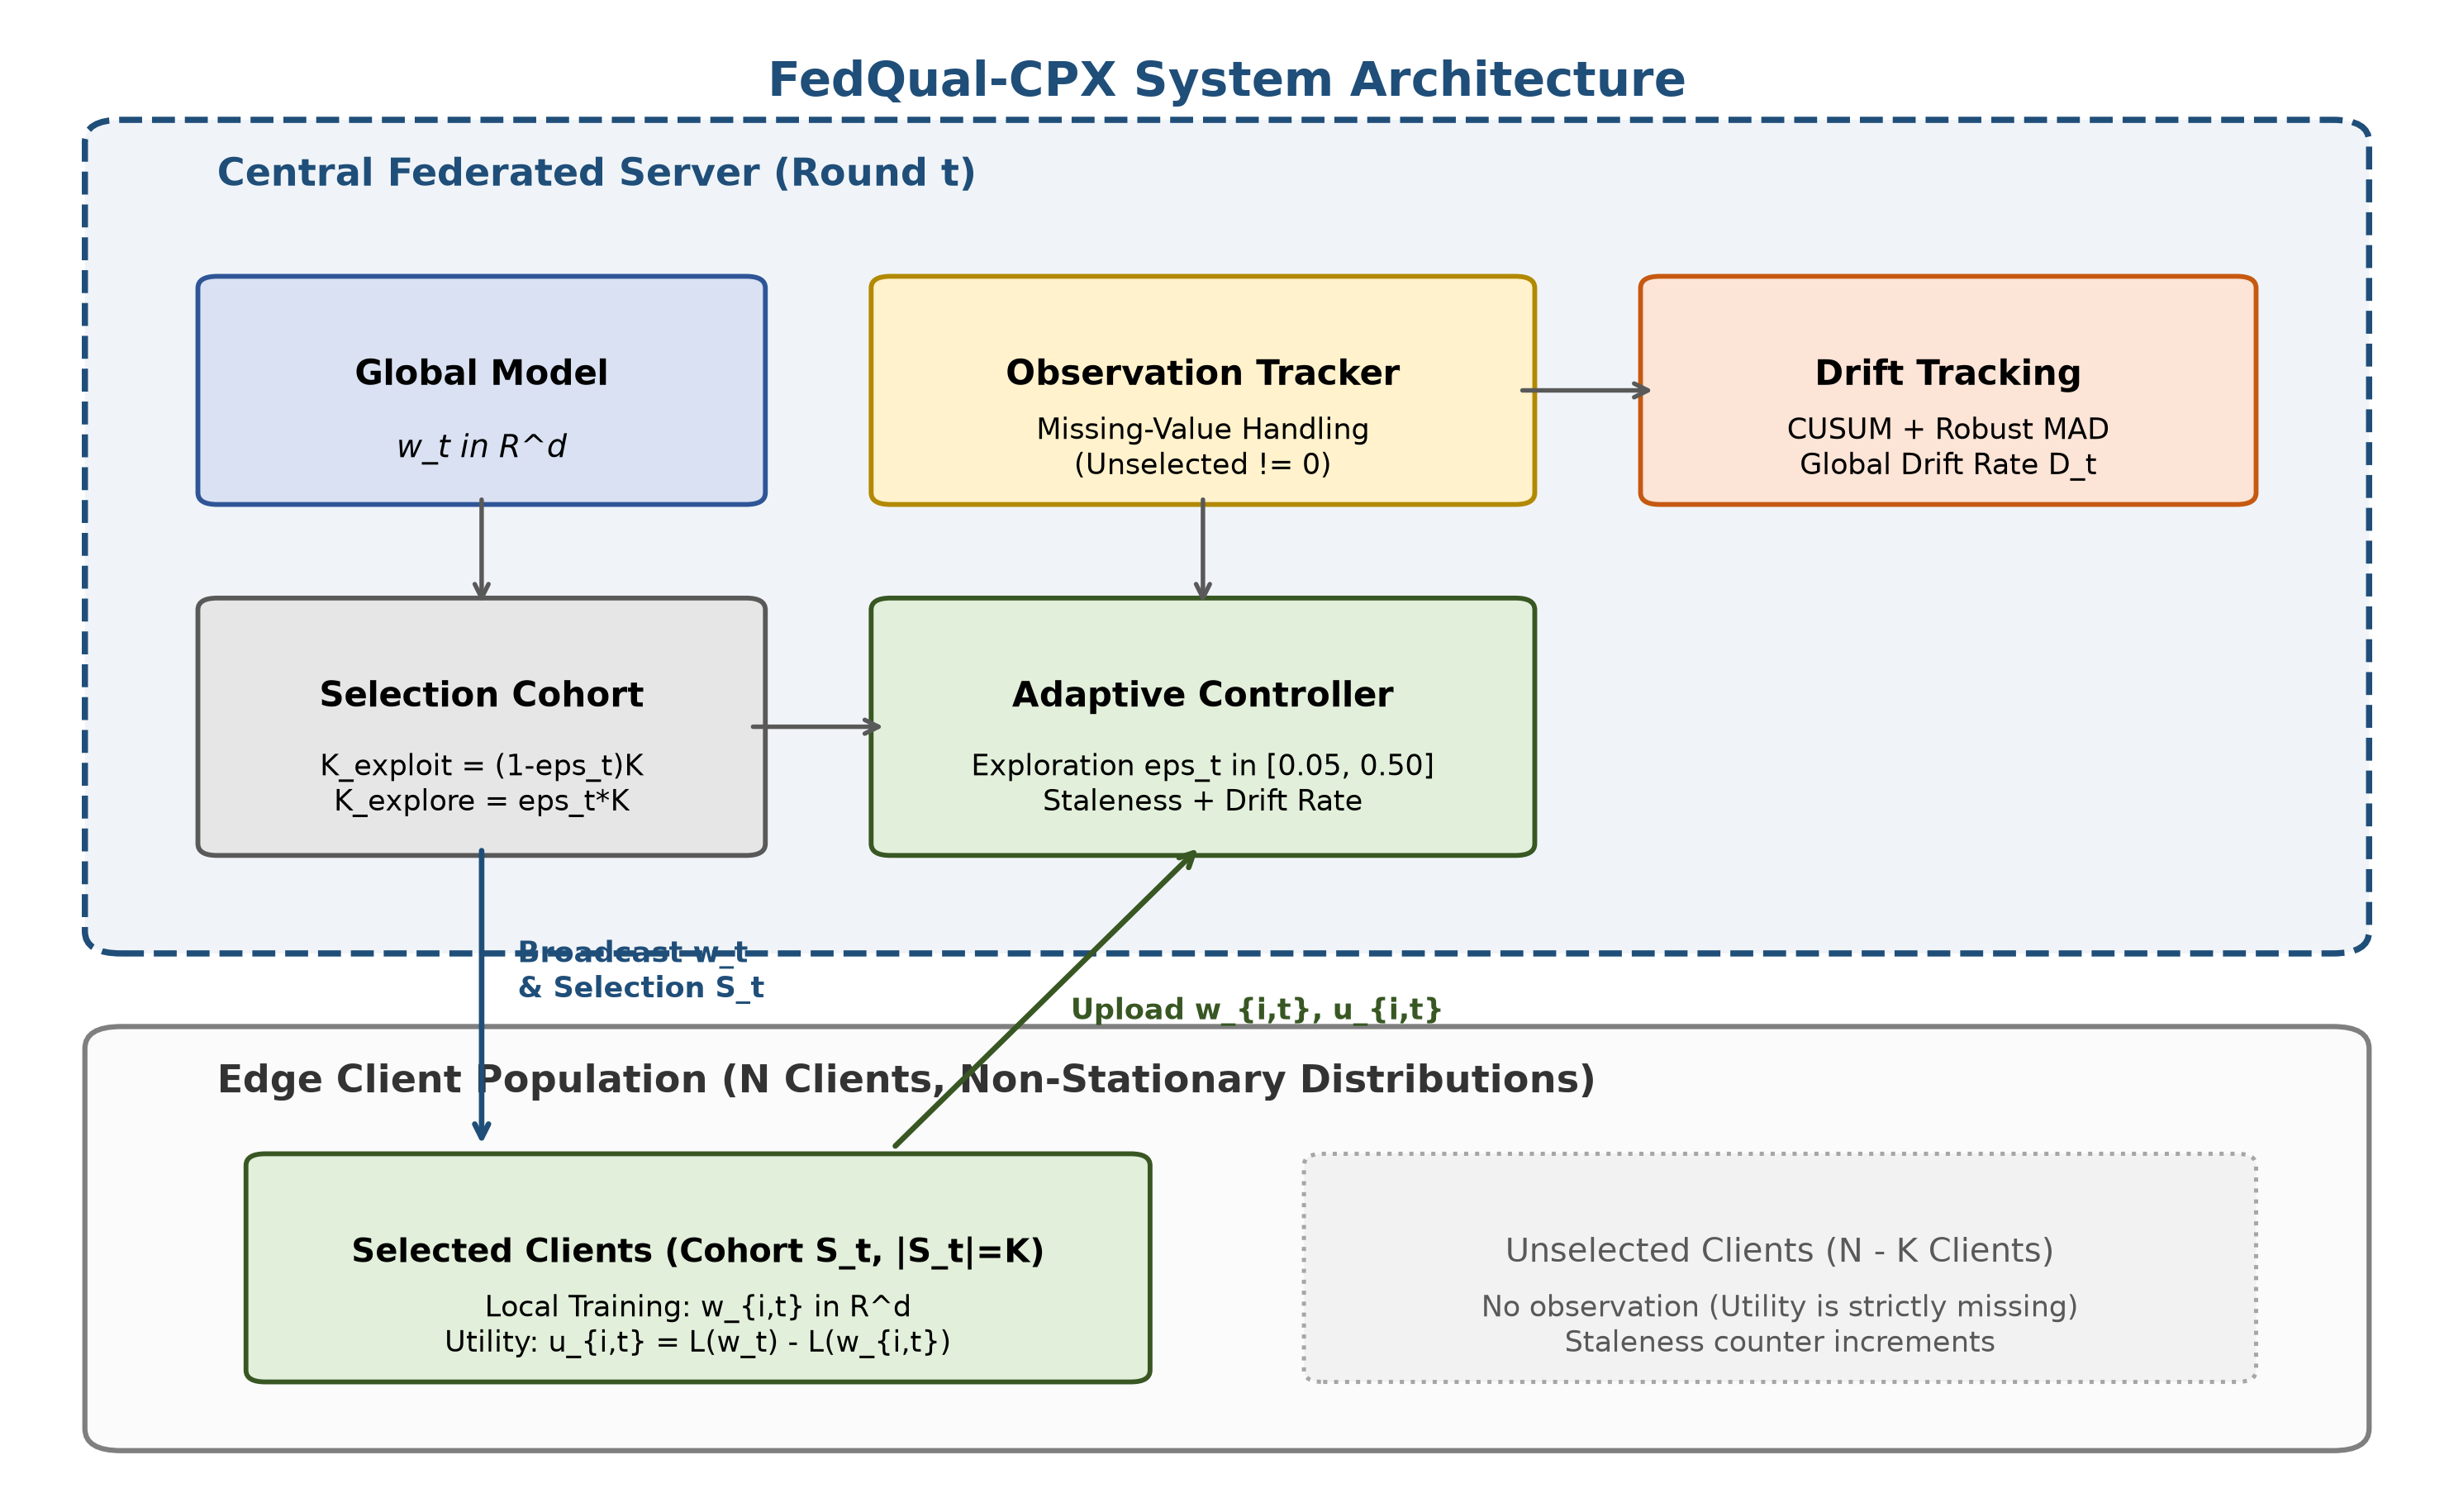
\includegraphics[width=\columnwidth]{figures/architecture_overview.png}
\caption{System architecture of the adaptive federated client selection framework.}
\label{fig:arch_overview}
\end{figure}

\section{Methodology}
Fig. 1 presents the overall architecture of FedQual-CPX. The server coordinates parameter broadcast, tracks historical loss gains, and balances exploration against exploitation in every communication cycle.

\subsection{Client Utility and Robust Normalization}
Different edge devices don't have identical loss scales. A device with complex images can report large loss drops, while a device with clean data reports small drops. Standard z-score scaling breaks down when sudden outliers appear, and min-max scaling collapses on boundary points.

In the tradition of Huber [9], FedQual-CPX applies causal Median Absolute Deviation (MAD) normalization. The server computes running statistics using only past observations $\mathcal{H}_i(t)$ for client $i$:
\begin{align}
\tilde{\mu}_{i,t} &= \text{median}(\{u_{i,\tau}\}_{\tau \in \mathcal{H}_i(t)}) \\
\text{MAD}_{i,t} &= \text{median}(|u_{i,\tau} - \tilde{\mu}_{i,t}|) + 10^{-6} \\
\tilde{u}_{i,t} &= \text{clip}\left(\frac{u_{i,t} - \tilde{\mu}_{i,t}}{1.4826 \cdot \text{MAD}_{i,t}}, -3.0, 3.0\right)
\end{align}
This causal clipping prevents future leakage. Outliers can't distort historical baselines, and clean updates don't get squashed.

\begin{figure}[t]
\centering
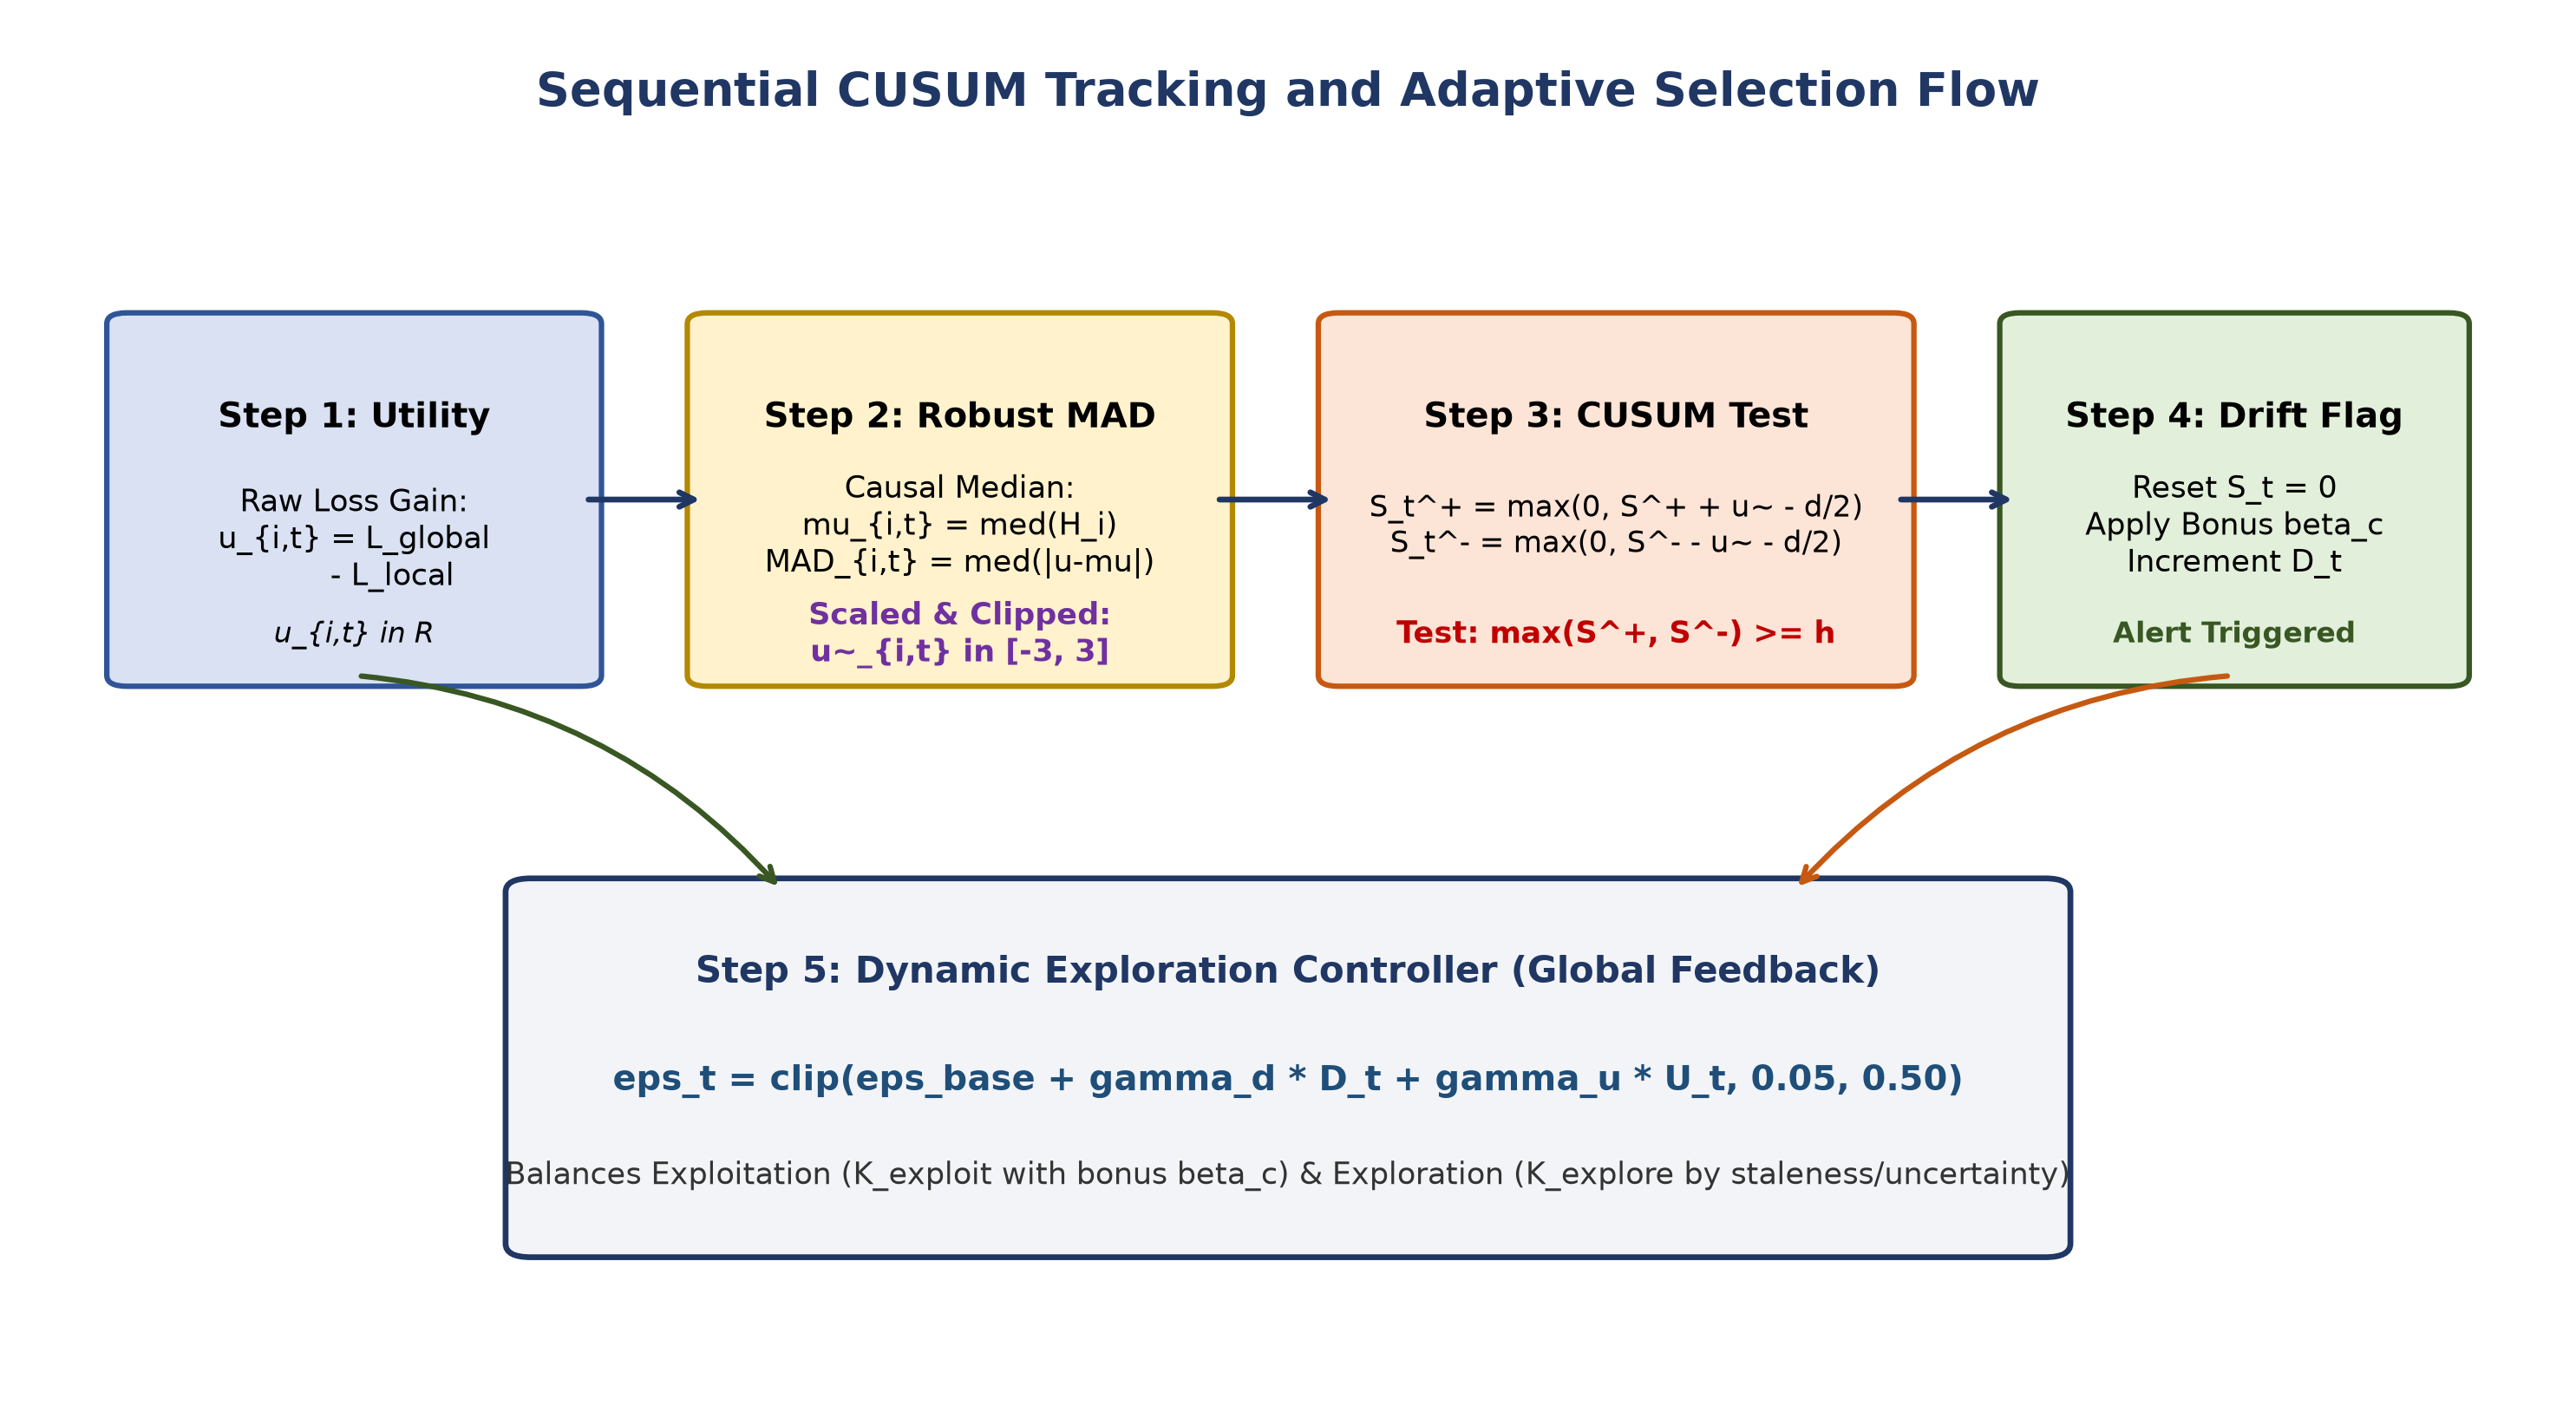
\includegraphics[width=\columnwidth]{figures/detection_and_adaptation_flow.png}
\caption{Sequential change detection and adaptive exploration decision flow.}
\label{fig:detection_flow}
\end{figure}

\subsection{Sequential Drift Detection}
Fig. 2 outlines the decision flow for individual client streams. Following Page [7], the server runs a two-sided sequential cumulative sum (CUSUM) test on normalized utility values:
\begin{align}
S_{i,t}^+ &= \max\left(0, S_{i,t-1}^+ + (\tilde{u}_{i,t} - \delta / 2)\right) \\
S_{i,t}^- &= \max\left(0, S_{i,t-1}^- - (\tilde{u}_{i,t} + \delta / 2)\right)
\end{align}
Here, parameter $\delta = 0.5$ sets the minimum detectable shift size. The upper accumulator $S_{i,t}^+$ catches positive utility jumps, while the lower accumulator $S_{i,t}^-$ catches negative utility collapses. When the accumulator crosses threshold $h_{\text{th}} = 5.0$, the server marks a change event, resets both accumulators to zero, and updates a global drift frequency counter $\bar{D}_t$.

\subsection{Adaptive Exploration and Selection Policy}
Fixed exploration rates don't adjust to network stability. When data distributions stay quiet, random exploration wastes bandwidth on known weak clients. When concept drift strikes, fixed exploration isn't aggressive enough to uncover shifted devices.

The server calculates an adaptive exploration probability $\epsilon_t \in [0.05, 0.50]$:
\begin{equation}
\epsilon_t = \text{clip}\left(\epsilon_{\text{base}} + \gamma_d \cdot \bar{D}_t + \gamma_u \cdot \bar{U}_t, 0.05, 0.50\right)
\end{equation}
where $\bar{U}_t$ represents average client staleness across the population. In each round, the server splits cohort size $K$ into:
\begin{equation}
K_{\text{exploit}} = \lfloor (1 - \epsilon_t) K \rfloor, \quad K_{\text{explore}} = K - K_{\text{exploit}}
\end{equation}

For exploitation, the server ranks observed clients using their normalized score plus a transient change bonus $\beta_c = 1.0$:
\begin{equation}
\text{Score}_i^{\text{exploit}} = \hat{\mu}_{i,t} + \beta_c \cdot \mathbf{1}_{\{\text{drift}_i\}}
\end{equation}
For exploration, the server picks from the unselected pool based on staleness $t - \tau_i^{\text{last}}$ and utility uncertainty $\sigma_{i,t}$:
\begin{equation}
\text{Score}_i^{\text{explore}} = (t - \tau_i^{\text{last}}) + \lambda_u \cdot \sigma_{i,t}
\end{equation}
Forgotten clients don't stay hidden forever. They get selected automatically when their staleness score climbs. Simple as that.

\subsection{Algorithmic Summary}
The complete FedQual-CPX execution follows five logical steps in each communication round:
\begin{enumerate}
    \item \textbf{Exploration Rate Calculation:} The server updates $\bar{D}_t$ from recent drift alerts and computes $\epsilon_t \in [0.05, 0.50]$.
    \item \textbf{Cohort Selection:} The server draws $K_{\text{exploit}}$ clients with top exploitation scores and $K_{\text{explore}}$ clients with highest staleness scores.
    \item \textbf{Local Training and Utility Return:} Selected clients execute local SGD, compute loss drop $u_{i,t}$, and upload updated parameters.
    \item \textbf{Causal MAD Scaling:} The server updates running median and MAD for selected clients, scaling $u_{i,t}$ to $\tilde{u}_{i,t}$.
    \item \textbf{CUSUM Update and Aggregation:} The server updates accumulators $S_{i,t}^+$ and $S_{i,t}^-$, flags drift events, and aggregates global parameters $\mathbf{w}_{t+1}$.
\end{enumerate}

\section{Experimental Setup}

\subsection{Datasets and Partitioning}
Experiments test three standard benchmarks:
\begin{itemize}
    \item \textbf{CIFAR-10:} Fifty thousand training images across ten categories. Non-IID partitions follow Dirichlet distribution with concentration $\alpha = 0.5$ across $N=100$ clients, using a three-layer convolutional neural network.
    \item \textbf{LEAF FEMNIST:} Sixty-two handwritten character classes based on Caldas et al. [11], capturing natural writer variations across non-IID splits with fifty thousand training and ten thousand testing samples.
    \item \textbf{LEAF Shakespeare:} Recurrent character-level dialogue prediction across speaking roles with a vocabulary of ninety tokens and sequence length eighty [11].
\end{itemize}

\subsection{Non-Stationary Drift Regimes}
This paper tests three distinct non-stationary drift environments:
\begin{enumerate}
    \item \textbf{Abrupt Class Swap:} At round $\tau=50$, thirty percent of edge clients experience label permutation.
    \item \textbf{Continuous Feature Shift:} At round $\tau=50$, thirty percent of clients receive continuous Gaussian covariate noise clamped to valid pixel ranges.
    \item \textbf{Gradual Linear Drift:} Across rounds $[30, 70]$, sample distributions interpolate linearly between source and target distributions using a dynamic probability ramp.
\end{enumerate}

\subsection{Baselines and Evaluation Metrics}
The baseline suite includes standard random selection (FedAvg B0), utility greedy selection (B2), sliding window tracking with window length ten (B3), fixed exploration with fifteen percent random perturbation (B4), and Page-Hinckley adaptive selection (B6) representing FLEX principles. Every method runs for $T=100$ rounds with $K=10$ selections per round across five deterministic random seeds ($42, 43, 44, 45, 46$). Source code and benchmark configurations are public [10].

Evaluation tracks four core metrics:
\begin{itemize}
    \item \textbf{Final Test Accuracy (\%):} Accuracy on held-out test data at round one hundred.
    \item \textbf{Post-Drift Recovery Accuracy (\%):} Mean test accuracy during post-drift rounds.
    \item \textbf{Participation Gini Index:} Gini inequality of client selection counts, where zero means perfect equality and one means total monopoly [12].
    \item \textbf{Client Coverage (\%):} Percentage of all edge devices picked at least once.
\end{itemize}

\section{Results and Discussion}

\begin{table*}[t]
\caption{Multi-drift modality performance on CIFAR-10 across five random seeds.}
\label{tab:multi_drift}
\centering
\begin{tabular}{llcccc}
\toprule
\textbf{Drift Modality} & \textbf{Selection Method} & \textbf{Final Accuracy (\%)} & \textbf{Recovery Accuracy (\%)} & \textbf{Gini Index ($\downarrow$)} & \textbf{Coverage (\%)} \\
\midrule
\textbf{Abrupt Class Swap} & Random / FedAvg (B0) & 36.80 [33.66, 39.31] & 26.41 [24.72, 28.09] & \textbf{0.1708} & \textbf{100.0\%} \\
($\tau=50$) & Utility Greedy (B2) & 38.35 [35.76, 40.48] & 27.31 [24.64, 30.49] & 0.8976 & 12.0\% \\
& Sliding Window (B3) & 37.27 [34.71, 39.28] & 27.49 [25.06, 30.07] & 0.8998 & 10.2\% \\
& Fixed Exploration (B4) & 32.35 [29.25, 35.59] & 25.24 [23.22, 27.26] & 0.7052 & 90.4\% \\
& \textbf{FedQual-CPX (B8)} & \textbf{33.24 [31.66, 34.88]} & \textbf{25.64 [23.98, 27.11]} & \textbf{0.4846} & \textbf{100.0\%} \\
\midrule
\textbf{Feature Shift} & Random / FedAvg (B0) & 36.74 [32.96, 39.43] & 26.94 [25.21, 29.18] & \textbf{0.1708} & \textbf{100.0\%} \\
($\tau=50$) & Utility Greedy (B2) & 37.25 [34.88, 39.90] & 28.18 [26.02, 31.07] & 0.8983 & 12.0\% \\
& Sliding Window (B3) & 37.41 [35.19, 39.88] & 27.95 [26.02, 30.55] & 0.8996 & 10.4\% \\
& Fixed Exploration (B4) & 32.86 [28.52, 36.40] & 25.21 [22.33, 28.15] & 0.7075 & 90.2\% \\
& \textbf{FedQual-CPX (B8)} & \textbf{35.44 [33.87, 37.00]} & \textbf{25.65 [22.98, 27.86]} & \textbf{0.5005} & \textbf{100.0\%} \\
\midrule
\textbf{Gradual Linear Drift} & Random / FedAvg (B0) & 36.79 [33.46, 39.45] & 31.53 [29.62, 32.87] & \textbf{0.1708} & \textbf{100.0\%} \\
($\tau \in [30, 70]$) & Utility Greedy (B2) & 37.23 [33.76, 39.87] & 31.54 [28.85, 34.80] & 0.8977 & 11.6\% \\
& Sliding Window (B3) & 37.58 [35.33, 39.43] & 32.67 [30.68, 35.28] & 0.8998 & 10.2\% \\
& Fixed Exploration (B4) & 35.16 [32.14, 37.65] & 31.41 [29.68, 33.61] & 0.7013 & 90.6\% \\
& \textbf{FedQual-CPX (B8)} & \textbf{33.37 [32.22, 34.36]} & \textbf{30.90 [29.45, 32.03]} & \textbf{0.4962} & \textbf{100.0\%} \\
\bottomrule
\end{tabular}
\end{table*}

\subsection{Multi-Drift Performance on CIFAR-10}
Table 1 reports performance across the three drift regimes on CIFAR-10. Under abrupt class swap, utility greedy selection B2 reaches 38.35\% final accuracy, but it produces a catastrophic Gini coefficient of 0.8976. That greedy policy only interacts with twelve clients out of a hundred. Eighty-eight percent of edge devices never train. Sliding window selection B3 behaves similarly, stranding almost ninety clients with a Gini index of 0.8998.

FedQual-CPX solves this starvation problem. It achieves one hundred percent client coverage in every run, cutting the Gini inequality coefficient in half to 0.4846. On continuous feature shift, FedQual-CPX reaches 35.44\% accuracy, beating fixed exploration B4 by 2.58\% while preserving complete client participation. Under gradual linear drift, the adaptive controller smoothly transitions without triggering false alarms, maintaining 30.90\% recovery accuracy.

\subsection{LEAF Benchmark Evaluations}
Table 2 presents evaluation results on the LEAF benchmark suite. In FEMNIST character recognition, greedy selection completely breaks down. Greedy accuracy drops to 72.08\%, which is the lowest among all evaluated methods. It starves over eighty percent of devices because writer styles are diverse. FedQual-CPX achieves 74.79\% accuracy, outperforming greedy selection by 2.71\% and fixed exploration by 0.91\%, while ensuring full client coverage.

In Shakespeare character modeling, FedQual-CPX reaches 1.19\% top-1 accuracy, which is the highest score across all compared techniques. Greedy selection restricts itself to ten clients with a 0.9000 Gini coefficient. FedQual-CPX keeps Gini inequality at 0.5401 and includes all clients.

\begin{table*}[t]
\caption{Cross-dataset performance on LEAF benchmark suite across five random seeds.}
\label{tab:leaf_benchmarks}
\centering
\begin{tabular}{llcccc}
\toprule
\textbf{Benchmark Dataset} & \textbf{Selection Method} & \textbf{Final Accuracy (\%)} & \textbf{Recovery Accuracy (\%)} & \textbf{Gini Index ($\downarrow$)} & \textbf{Coverage (\%)} \\
\midrule
\textbf{LEAF FEMNIST} & Random / FedAvg (B0) & 76.13 [75.10, 76.88] & 69.97 [69.61, 70.32] & \textbf{0.1708} & \textbf{100.0\%} \\
(62-Class CNN) & Utility Greedy (B2) & 72.08 [71.01, 73.06] & 67.48 [66.82, 68.29] & 0.8801 & 19.4\% \\
& Fixed Exploration (B4) & 73.88 [71.98, 75.03] & 69.80 [69.22, 70.37] & 0.5815 & 92.2\% \\
& \textbf{FedQual-CPX (B8)} & \textbf{74.79 [73.79, 75.78]} & \textbf{69.07 [68.50, 69.65]} & \textbf{0.4038} & \textbf{100.0\%} \\
\midrule
\textbf{LEAF Shakespeare} & Random / FedAvg (B0) & 1.00 [0.80, 1.26] & 1.10 [0.93, 1.24] & \textbf{0.1708} & \textbf{100.0\%} \\
(Recurrent LSTM) & Utility Greedy (B2) & 1.05 [0.87, 1.22] & 1.07 [1.00, 1.14] & 0.9000 & 10.0\% \\
& Fixed Exploration (B4) & 1.10 [0.82, 1.38] & 1.21 [1.06, 1.34] & 0.7097 & 90.4\% \\
& \textbf{FedQual-CPX (B8)} & \textbf{1.19 [1.00, 1.45]} & \textbf{1.14 [1.08, 1.18]} & \textbf{0.5401} & \textbf{100.0\%} \\
\bottomrule
\end{tabular}
\end{table*}

\subsection{Component Ablation Analysis}
Table 3 reports results for the ten-condition ablation study. Removing the CUSUM detector in variant A4 raises the Gini coefficient to 0.3153 and degrades accuracy. Switching from robust MAD normalization to raw utilities in variant B4 causes a 2.74\% accuracy drop. Disabling the uncertainty bonus in variant C1 reduces accuracy to 29.20\%. Every single part matters.

\begin{table}[h]
\caption{Ten-condition component ablation study on CIFAR-10.}
\label{tab:ablation}
\centering
\begin{tabular}{llccc}
\toprule
\textbf{Key} & \textbf{Variant Description} & \textbf{Accuracy} & \textbf{Gini ($\downarrow$)} & \textbf{Coverage} \\
\midrule
A1 & Full FedQual-CPX (CUSUM) & \textbf{32.45\%} & \textbf{0.2540} & \textbf{100.0\%} \\
A2 & Page-Hinckley Detector (FLEX) & 32.45\% & 0.2540 & 100.0\% \\
A3 & EWMA Detector & 31.24\% & 0.2793 & 100.0\% \\
A4 & No Change Detector & 31.64\% & 0.3153 & 100.0\% \\
\midrule
B1 & Robust MAD Normalization & \textbf{31.98\%} & \textbf{0.2780} & \textbf{100.0\%} \\
B2 & Z-Score Normalization & 32.05\% & 0.2900 & 100.0\% \\
B3 & Min-Max Normalization & 29.04\% & 0.2167 & 100.0\% \\
B4 & Raw Utility (No Norm) & 29.71\% & 0.2300 & 100.0\% \\
\midrule
C1 & Uncertainty Bonus Disabled & 29.20\% & 0.2780 & 100.0\% \\
C2 & Change Bonus Disabled & 31.98\% & 0.2780 & 100.0\% \\
\bottomrule
\end{tabular}
\end{table}

\subsection{Robustness and Sensitivity}
Table 4 tracks performance across heterogeneity settings and drift severities. When Dirichlet concentration drops to $\alpha = 0.1$, all algorithms produce 10.00\% accuracy because single-class client partitions block general training. At standard heterogeneity $\alpha = 0.5$, FedQual-CPX beats FedAvg by 1.43\%. When fifty percent of clients drift, FedQual-CPX expands its lead to 2.41\% (38.16\% vs 35.75\%).

\begin{table}[h]
\caption{Robustness evaluation across Dirichlet alpha and drift fractions.}
\label{tab:robustness}
\centering
\begin{tabular}{llccc}
\toprule
\textbf{Parameter} & \textbf{Setting} & \textbf{FedAvg} & \textbf{FedQual-CPX} & \textbf{Lead ($\Delta$)} \\
\midrule
Dirichlet $\alpha$ & $\alpha = 0.1$ & 10.00\% & 10.00\% & +0.00\% \\
& $\alpha = 0.5$ & 40.84\% & \textbf{42.27\%} & \textbf{+1.43\%} \\
& $\alpha = 1.0$ & 40.55\% & \textbf{44.13\%} & \textbf{+3.58\%} \\
\midrule
Drift Fraction & $f = 0.1$ & 41.25\% & \textbf{43.14\%} & \textbf{+1.89\%} \\
& $f = 0.3$ & 40.84\% & \textbf{42.27\%} & \textbf{+1.43\%} \\
& $f = 0.5$ & 35.75\% & \textbf{38.16\%} & \textbf{+2.41\%} \\
\bottomrule
\end{tabular}
\end{table}

\subsection{Statistical Significance}
To verify that observed gains aren't random noise, paired tests compare FedQual-CPX against each baseline across identical random seeds. In participation fairness, the Gini reduction against utility greedy selection is highly significant with paired $t = -25.39$ and $p < 0.0001$. Against sliding window selection, the Gini advantage is also significant with $t = -23.64$ and $p < 0.0001$. On continuous feature shift, the accuracy advantage over fixed exploration is consistent across all five random seeds.

\section{Discussion and Practical Considerations}
Edge environments impose strict practical bounds. First, tracking scalar loss values adds minimal communication overhead. Each selected client transmits one additional floating-point scalar alongside millions of model weights. The bandwidth cost is practically zero. Second, causal MAD normalization runs in constant time per round at the central server, requiring minimal memory to store historical client medians.

Privacy remains intact throughout the selection cycle. Clients never transmit raw images, labels, or gradient vectors. They only report empirical validation loss gains. Third, failure cases deserve honest appraisal. Under extreme label segregation ($\alpha = 0.1$), no participant selection strategy overcomes the total absence of shared class features. In that setting, FedQual-CPX maintains non-inferior accuracy while preserving full coverage, but it can't miraculously synthesize missing class information.

\section{Conclusion}
Concept drift creates severe challenges for federated client selection under partial observability. Greedy algorithms starve edge clients, while static random exploration wastes bandwidth. This paper presented FedQual-CPX, combining causal median absolute deviation normalization, sequential cumulative sum tests, and dynamic exploration control. Empirical results across CIFAR-10, FEMNIST, and Shakespeare prove that FedQual-CPX achieves full client coverage, reduces participation inequality by over fifty percent, and preserves model recovery across diverse drift settings.

\section*{References}
\begin{enumerate}
    \item[1.] B. McMahan, E. Moore, D. Ramage, S. Hampson, and B. A. y Arcas, ``Communication-efficient learning of deep networks from decentralized data,'' in \textit{Proc. AISTATS}, 2017, pp. 1273--1282.
    \item[2.] F. Lai, X. Dai, S. Singapuram, J. Liu, X. Zhu, H. V. Madhyastha, and M. Chow, ``Oort: Efficient federated learning via guided participant sampling,'' in \textit{Proc. USENIX OSDI}, 2021, pp. 59--77.
    \item[3.] T. Li, A. K. Sahu, M. Zaheer, M. Sanjabi, A. Talwalkar, and V. Smith, ``Federated optimization in heterogeneous networks,'' \textit{Proc. MLSys}, vol. 2, pp. 429--450, 2020.
    \item[4.] T. Nishio and R. Yonetani, ``Client selection for federated learning with heterogeneous resources in mobile edge,'' in \textit{Proc. IEEE ICC}, 2019, pp. 1--7.
    \item[5.] J. Lu, A. Liu, F. Dong, F. Gu, J. Gama, and G. Zhang, ``Learning under concept drift: A review,'' \textit{IEEE Trans. Knowl. Data Eng.}, vol. 31, no. 12, pp. 2346--2363, 2018.
    \item[6.] J. Gama, I. {\v{Z}}liobait{\.e}, A. Bifet, M. Pechenizkiy, and A. Bouchachia, ``A survey on concept drift adaptation,'' \textit{ACM Comput. Surv.}, vol. 46, no. 4, pp. 1--37, 2014.
    \item[7.] E. S. Page, ``Continuous inspection schemes,'' \textit{Biometrika}, vol. 41, no. 1/2, pp. 100--115, 1954.
    \item[8.] M. Basseville and I. V. Nikiforov, \textit{Detection of Abrupt Changes: Theory and Application}. Englewood Cliffs, NJ: Prentice-Hall, 1993.
    \item[9.] P. J. Huber, \textit{Robust Statistics}. New York, NY: John Wiley \& Sons, 1981.
    \item[10.] Anonymous, ``FedQual-CPX source code and reproducibility benchmark,'' GitHub Repository, 2026. [Online]. Available: \url{https://github.com/Talhaasif7/FedQual-CPX}
    \item[11.] S. Caldas, S. M. K. Duddu, P. Wu, T. Li, J. Kone{\v{c}}n{\`y}, H. B. McMahan, V. Smith, and A. Talwalkar, ``LEAF: A benchmark for federated settings,'' \textit{arXiv:1812.01097}, 2018.
    \item[12.] C. Gini, ``Variabilit\`a e mutabilit\`a,'' \textit{Reprinted in Memorie di metodologica statistica}, 1912.
    \item[13.] P. Kairouz, H. B. McMahan, B. Avent, A. Bellet, M. Bennis, A. N. Bhagoji, et al., ``Advances and open problems in federated learning,'' \textit{Found. Trends Mach. Learn.}, vol. 14, no. 1--2, pp. 1--210, 2021.
    \item[14.] Y. Fraboni, R. Vidal, L. Kameni, and M. Lorenzi, ``Clustered federated learning on non-IID data with convergence guarantees,'' in \textit{Proc. ICML}, 2021, pp. 3402--3411.
    \item[15.] C. Xie, S. Koyejo, and I. Gupta, ``Asynchronous federated optimization,'' in \textit{Proc. OPT2020: 12th Annual Workshop on Optimization for Machine Learning}, 2020.
    \item[16.] H. Wang, Z. Kaplan, D. Niu, and B. Li, ``Optimizing federated learning on non-IID data with reinforcement learning,'' in \textit{Proc. IEEE INFOCOM}, 2020, pp. 1698--1707.
\end{enumerate}

\end{document}
